% Prof. Dr. Ausberto S. Castro Vera
% UENF - CCT - LCMAT - Curso de Ci\^{e}ncia da Computa\c{c}\~{a}o
% Campos, RJ,  2022
% Disciplina: An\'{a}lise e Projeto de Sistemas
% Aluno:

\chapterimage{analise.png} % Table of contents heading image
\chapter{Etapa de An\'{a}lise}

Neste capítulo, descrevemos tudo o que é necessário para o correto funcionamento do sistema, como a análise do sistema, que é composta pela coleta e apresentação de requisitos, seleção de stakeholders, entrevistas, casos de uso, diagramas de fluxo de dados, e diagrama de entidade e relacionamentos. De modo a  proporcionar o entendimento das funções que o sistema realizará.



\section{Requisitos do Sistema}







\begin{enumerate}
      %%%%%%%%%%%%%%%%%%%%%%%%%%%%%%%%%%%%%%%%%%%%
      \item \textbf{Segurança do sistema;}

            \begin{enumerate}
                  \item O sistema deve ser capaz de prevenir erros e perdas de dados.
                        \begin{enumerate}
                              \item Verificação de cadastro do usuário no login;
                              \item Verificação de CAPTCHA;
                              \item Verificação de permissões do perfil do usuário para acessar certos componentes do sistema;
                              \item Emissão de alertas caso o usuário tente executar uma função de maneira incorreta;



                        \end{enumerate}
            \end{enumerate}
            %%%%%%%%%%%%%%%%%%%%%%%%%%%%%%%
      \item \textbf{Sincronização entre veículos;}
            \begin{enumerate}

                  \item	O sistema deve estar sempre sincronizado de
                        forma a prevenir erros de comunicação.
                        \begin{enumerate}
                              \item Acesso às informações entre qualquer veículo da empresa;
                              \item Sincronização dos dados;
                              \item Comunicação entre veículos, para troca de veículos em casa de problemas.

                        \end{enumerate}
            \end{enumerate}
            %%%%%%%%%%%%%%%%%%%%%%%%%%%%%%%
      \item \textbf{Manual do usuário;}
            \begin{enumerate}

                  \item	No manual usuário terá todas as informações das funções do
                        sistema.

                        \begin{enumerate}
                              \item Descrição do que o sistema é capaz de fazer;
                              \item Informações das versões;
                              \item Informações dos desenvolvedores do sistema.

                        \end{enumerate}
            \end{enumerate}
            %%%%%%%%%%%%%%%%%%%%%%%%%%%%%%%
            %%%%%%%%%%%%%%%%%%%%%%%%%%%%%%%
      \item \textbf{Programa de gerenciamento de finanças da empresa;}
            \begin{enumerate}

                  \item	O sistema irá permitir visualizar a situação financeira da empresa, podendo também
                        gerar relatórios sobre essas finanças.

                        \begin{enumerate}
                              \item Emissão de relatórios;
                              \item Visão geral das finanças;
                              \item Salvar relatórios;
                              \item Visualização dos lucros e gastos;
                              \item Relatório do valor gerado por cada veículo da empresa;
                              \item Gastos com terceirizadas, combustíveis, manutenções.

                        \end{enumerate}
            \end{enumerate}
            %%%%%%%%%%%%%%%%%%%%%%%%%%%%%%%
      \item \textbf{Disponibilidade dos veículos;}
            \begin{enumerate}

                  \item	O sistema deve ser capaz de localizar e saber a disponibilidade do veículo da empresa.
                        \begin{enumerate}
                              \item Busca pelo veículo no sistema;

                              \item Classificação dos veículos podem ser de maneira customizadas;
                              \item Emitir alerta se o veículo estiver indisponível e disponível;
                              \item Mostra relatório do status geral do veiculo como: Nivel de combustivel, tempo estimado para a próxima parada de manutenção.

                        \end{enumerate}
            \end{enumerate}
            %%%%%%%%%%%%%%%%%%%%%%%%%%%%%%%
      \item \textbf{Aplicativo da empresa;}
            \begin{enumerate}

                  \item	Deverá ter as funções necessárias para a solicitação de veículo, e gestão da viagem.
                        \begin{enumerate}
                              \item Opção de agendar/solicitar/cancelar viagens;
                              \item Acompanhamento do andamento da viagem;
                              \item Visualização de histórico de viagens;
                              \item Escolher forma de pagamento;
                              \item Escolher tipo de viagem;
                              \item Escolher local de embarque e de destino;
                              \item  Opção de escolha do veículo;
                              \item O sistema deve solicitar ao usuário a quantidade de passageiros que irão fazer a viagem;
                              \item O sistema deve mostrar a estimativa de tempo da viagem;
                              \item O sistema deve mostrar ao usuário o valor total da viagem;
                              \item O sistema deve dar a opção de cancelar a viagem antes de chegar ao destino final informado;
                              \item O sistema deve dar opção de mudar o destino final com a viagem em andamento.


                        \end{enumerate}
            \end{enumerate}
            %%%%%%%%%%%%%%%%%%%%%%%%%%%%%%%
            %\item ----;
            %       \begin{enumerate}

            %        \item	----

            %         \begin{enumerate}
            %                     \item ----
            %                  \item ---;
            %               \item ----.

            %        \end{enumerate}
            %\end{enumerate}

            %%%%%%%%%%%%%%%%%%%%%%%%%%%%%%%
      \item \textbf{Backup do sistema;}
            \begin{enumerate}

                  \item	Haverá backup do sistema de forma constante.
                        \begin{enumerate}
                              \item O Backup deverá receber os dados de todos os sistema da empresa;
                              \item O Backup terá redundância de dados.


                        \end{enumerate}
            \end{enumerate}

            %%%%%%%%%%%%%%%%%%%%%%%%%%%%%%%
      \item \textbf{Receber feedback dos usuários;}
            \begin{enumerate}

                  \item O aplicativo deverá ter opção de receber feedback dos usuários.
                        \begin{enumerate}
                              \item O feedback deve conter análise de sentimentos feita por IA;
                              \item O feedback deve constar a avaliação que o usuário deu para a viagem;
                              \item O feedback deve constar data e hora em que foi gerado.

                        \end{enumerate}
            \end{enumerate}

            %%%%%%%%%%%%%%%%%%%%%%%%%%%%%%%
      \item \textbf{Monitoramento 24h;}
            \begin{enumerate}

                  \item	O monitoramento das câmeras deverá ser feito por inteligência artificial.

                        \begin{enumerate}
                              \item Acompanhamento de todas as câmeras;
                              \item Controle de todas as câmeras;
                              \item Análise sentimental para compreender se o usuários está passando por alguma situação.

                        \end{enumerate}
            \end{enumerate}

            %%%%%%%%%%%%%%%%%%%%%%%%%%%%%%%
      \item \textbf{Treinamento de novos funcionários e colaboradores;}
            \begin{enumerate}

                  \item	Treinamento intensivo de novos funcionários e colaboradores a fim de substituição imediata.

                        \begin{enumerate}
                              \item Coleta de informações de funcionários e colaborador antigo;
                              \item Análise do antigo colaborador a fim de identificar os pontos principais que deverão ser remanejados para o novo funcionário;
                              \item Leitura do manual de treinamento;
                              \item Planejamento do treinamento;
                              \item Escolha apropriada do novo profissional a ser contratado;
                              \item Reunião para dúvidas e questionamentos;
                              \item Testes de entendimento aos requisitos do sistema;
                              \item Avaliação da experiência com o sistema da empresa;
                              \item Identificação de histórico do novo colaborador;
                              \item Finalização do treinamento e contratação.

                        \end{enumerate}
            \end{enumerate}

            %%%%%%%%%%%%%%%%%%%%%%%%%%%%%%%
      \item \textbf{Relatórios da empresa;}
            \begin{enumerate}

                  \item	Deverá ser realizado relatórios de maneira semanal e mensal das atividades da empresa.

                        \begin{enumerate}
                              \item Registro de todos os acessos;
                              \item Registro de todas as ações feitas com o sistema;
                              \item Registro dos acionamentos;
                              \item Ata de reuniões feitas;
                              \item Documentação de ações suspeitas identificadas;

                              \item Documentação de problemas com os veículos da empresa.
                        \end{enumerate}
            \end{enumerate}

            %%%%%%%%%%%%%%%%%%%%%%%%%%%%%%%


      \item \textbf{Servidores dedicados;}
            \begin{enumerate}

                  \item	O sistema deverá conter servidores dedicados para armazenamento dos dados do aplicativo, para backups dos bancos de dados.



            \end{enumerate}

            %%%%%%%%%%%%%%%%%%%%%%%%%%%%%%%
      \item \textbf {Equipamentos de redes;}
            \begin{enumerate}

                  \item	Será instalado equipamentos de rede para cada funcionário em modo remoto. Assim mantendo todos os colaboradores com acesso a internet.



            \end{enumerate}

            %%%%%%%%%%%%%%%%%%%%%%%%%%%%%%%

      \item \textbf{Equipamento de comunicação;}
            \begin{enumerate}

                  \item	Os colaboradores devem poder se comunicar uns com os outros para fins de notificação, atualização e monitoramento de casos. Desse modo, pode ocorrer a comunicação direta entre a equipe..



            \end{enumerate}

            %%%%%%%%%%%%%%%%%%%%%%%%%%%%%%%
      \item \textbf {Câmeras de segurança;}
            \begin{enumerate}

                  \item	Necessárias para o monitoramento interno dos veículos.



            \end{enumerate}

            %%%%%%%%%%%%%%%%%%%%%%%%%%%%%%%
      \item \textbf{Mobília;}
            \begin{enumerate}

                  \item	Será necessário alguns tipos de mobília para os funcionários.



            \end{enumerate}

            %%%%%%%%%%%%%%%%%%%%%%%%%%%%%%%
      \item \textbf{Gerenciamento de câmeras;}
            \begin{enumerate}

                  \item	As câmeras deverão ser operadas 24h apenas por colaboradores autorizados e propriamente credenciados.



            \end{enumerate}

            %%%%%%%%%%%%%%%%%%%%%%%%%%%%%%%
      \item \textbf{Gerenciamento dos dados armazenados;}
            \begin{enumerate}

                  \item	Os dados coletados  e produzidos só poderão ser acessados por meio de um protocolo emitido e assinado pelo(a) analista encarregado.



            \end{enumerate}

            %%%%%%%%%%%%%%%%%%%%%%%%%%%%%%%
      \item \textbf{Controle do fluxo de veículos em operação; }
            \begin{enumerate}

                  \item	O controle do fluxo de veículos em cada região deverá ser determinado com base na procura pelo mesmo.



            \end{enumerate}

            %%%%%%%%%%%%%%%%%%%%%%%%%%%%%%%
      \item \textbf{Acionamento das autoridades locais;}
            \begin{enumerate}

                  \item	Em casos extremos e necessários: encaminhamento de casos suspeitos para as autoridades superiores de cada estado.



            \end{enumerate}

            %%%%%%%%%%%%%%%%%%%%%%%%%%%%%%%
      \item \textbf{O acesso com login e senha;}
            \begin{enumerate}

                  \item	Nenhum cidadão ou demais funcionários além dos autorizados terão acesso ao sistema.


            \end{enumerate}

            %%%%%%%%%%%%%%%%%%%%%%%%%%%%%%%
      \item \textbf{Velocidade do sistema;}
            \begin{enumerate}

                  \item	O sistema deverá trabalhar com a melhor e mais rápida tecnologia existente.



            \end{enumerate}

            %%%%%%%%%%%%%%%%%%%%%%%%%%%%%%%
      \item \textbf{Analista de segurança da informação;}
            \begin{enumerate}

                  \item	É de extrema importância a contratação de analistas de segurança para fazer o gerenciamento do sistema.



            \end{enumerate}

            %%%%%%%%%%%%%%%%%%%%%%%%%%%%%%%
      \item \textbf{Programadores;}
            \begin{enumerate}

                  \item	 Fundamental a contratação de programadores para a implementação e manutenção do sistema.



            \end{enumerate}

            %%%%%%%%%%%%%%%%%%%%%%%%%%%%%%%
      \item \textbf{Gerente de Projetos;}
            \begin{enumerate}

                  \item	O gerente de projetos deverá ser contratado para auxiliar toda a equipe no remanejamento das atividades relacionadas à implementação.



            \end{enumerate}

            %%%%%%%%%%%%%%%%%%%%%%%%%%%%%%%
      \item \textbf{Equipe de manutenção;}
            \begin{enumerate}

                  \item	Realizará a manutenção preventiva dos equipamentos e manter todos em perfeito funcionamento.



            \end{enumerate}

            %%%%%%%%%%%%%%%%%%%%%%%%%%%%%%%
      \item \textbf{Manual do sistema e projeto;}
            \begin{enumerate}

                  \item	Para cada sistema e projeto deverá haver ver manual documentado para facilitar os seus usos em caso de dúvidas.



            \end{enumerate}

            %%%%%%%%%%%%%%%%%%%%%%%%%%%%%%%
      \item \textbf{Listagem de funcionários;}
            \begin{enumerate}

                  \item	É fundamental a existência de listagem de todos os funcionários da empresa.



            \end{enumerate}

            %%%%%%%%%%%%%%%%%%%%%%%%%%%%%%%
      \item \textbf{Imagens e resolução;}
            \begin{enumerate}

                  \item	As câmeras internas dos veículos da empresa deverão produzir imagens em alta definição.



            \end{enumerate}

            %%%%%%%%%%%%%%%%%%%%%%%%%%%%%%%
      \item \textbf{Backup de imagens e vídeos; }
            \begin{enumerate}

                  \item	Os dados das câmeras deverão ser armazenados no banco de dados por um período de 30 dias. Entretanto, mediante a solicitação jurídica as imagens deverão ser mantidas armazenadas até a resolução do caso.


            \end{enumerate}

            %%%%%%%%%%%%%%%%%%%%%%%%%%%%%%%
      \item \textbf{Histórico de acesso;}
            \begin{enumerate}

                  \item	Deverá ser armazenado no banco de dados, todos os acessos a dados da empresa.



            \end{enumerate}

            %%%%%%%%%%%%%%%%%%%%%%%%%%%%%%%
      \item \textbf{Manual de treinamento de colaboradores;}
            \begin{enumerate}

                  \item	É fundamental a criação de documento base para a aplicação de treinamento para funcionários e colaboradores.



            \end{enumerate}

            %%%%%%%%%%%%%%%%%%%%%%%%%%%%%%%
      \item \textbf{Manutenção preventiva;}
            \begin{enumerate}

                  \item	Deverá ser realizada manutenção preventiva a cada 1 mês em todos os veículos da empresa.



            \end{enumerate}

            %%%%%%%%%%%%%%%%%%%%%%%%%%%%%%%
      \item \textbf{Relatórios semanais;}
            \begin{enumerate}

                  \item	Será documentado e produzido um relatório sobre as ocorrências.



            \end{enumerate}

            %%%%%%%%%%%%%%%%%%%%%%%%%%%%%%%

      \item \textbf{Em caso de acidentes; }
            \begin{enumerate}

                  \item	Havendo acidentes com os veículos da empresa será solicitado o suporte das autoridades locais, e uma equipe terceirizada irá ser destinada ao local.



            \end{enumerate}

            %%%%%%%%%%%%%%%%%%%%%%%%%%%%%%%

      \item \textbf{Em caso de problemas em algum veículo da empresa;}
            \begin{enumerate}

                  \item	Se houver algum problema com um veículo e um passageiro estiver no veículo. Um novo veículo da empresa será destinado para o local para continuar com a viagem do usuário.



            \end{enumerate}

            %%%%%%%%%%%%%%%%%%%%%%%%%%%%%%%
      \item \textbf{Sincronização de digitais na nuvem;}


            %%%%%%%%%%%%%%%%%%%%%%%%%%%%%%%
      \item \textbf{Arquivos de Vídeo;}


            %%%%%%%%%%%%%%%%%%%%%%%%%%%%%%%
      \item \textbf{Arquivos de áudio;}


            %%%%%%%%%%%%%%%%%%%%%%%%%%%%%%%


      \item \textbf{Backup mensal;}


            %%%%%%%%%%%%%%%%%%%%%%%%%%%%%%%


      \item \textbf{Backup anual;}


            %%%%%%%%%%%%%%%%%%%%%%%%%%%%%%%


      \item \textbf{Dispositivo de escuta;}


            %%%%%%%%%%%%%%%%%%%%%%%%%%%%%%%


      \item \textbf{Tablet;}


            %%%%%%%%%%%%%%%%%%%%%%%%%%%%%%%


      \item \textbf{Workstation;}


            %%%%%%%%%%%%%%%%%%%%%%%%%%%%%%%


      \item \textbf{Cadastro de funcionários;}


            %%%%%%%%%%%%%%%%%%%%%%%%%%%%%%%


      \item \textbf{Cadastro de digitais;}


            %%%%%%%%%%%%%%%%%%%%%%%%%%%%%%%


      \item \textbf{Fiscalização de pessoas;}


            %%%%%%%%%%%%%%%%%%%%%%%%%%%%%%%


      \item \textbf{Capacitação dos funcionários;}


            %%%%%%%%%%%%%%%%%%%%%%%%%%%%%%%


      \item \textbf{Relatório do ano completo;}


            %%%%%%%%%%%%%%%%%%%%%%%%%%%%%%%


      \item \textbf{Histórico de navegação no sistema;}


            %%%%%%%%%%%%%%%%%%%%%%%%%%%%%%%


      \item \textbf{Funcionários autorizados a áreas restritas do sistema;}


            %%%%%%%%%%%%%%%%%%%%%%%%%%%%%%%


      \item \textbf{Código de conduta;}


            %%%%%%%%%%%%%%%%%%%%%%%%%%%%%%%


      \item \textbf{Normais da empresa;}


            %%%%%%%%%%%%%%%%%%%%%%%%%%%%%%%


      \item \textbf{Listagem de intervenção semanal;}


            %%%%%%%%%%%%%%%%%%%%%%%%%%%%%%%

      \item \textbf{Diagramas;}


            %%%%%%%%%%%%%%%%%%%%%%%%%%%%%%%

      \item \textbf{Orçamento;}


            %%%%%%%%%%%%%%%%%%%%%%%%%%%%%%%

      \item \textbf{Documentação detalhada do sistema;}


            %%%%%%%%%%%%%%%%%%%%%%%%%%%%%%%

      \item \textbf{Manual do usuário;}


            %%%%%%%%%%%%%%%%%%%%%%%%%%%%%%%

      \item \textbf{Equipamentos para localização dos veículos; }


            %%%%%%%%%%%%%%%%%%%%%%%%%%%%%%%

      \item \textbf{Sistema de controle;}


            %%%%%%%%%%%%%%%%%%%%%%%%%%%%%%%

      \item \textbf{Cadastro de novos recursos;}


            %%%%%%%%%%%%%%%%%%%%%%%%%%%%%%%
      \item \textbf{Programa de gerenciamento;}


            %%%%%%%%%%%%%%%%%%%%%%%%%%%%%%%
      \item \textbf{Engenheiro de software;}


            %%%%%%%%%%%%%%%%%%%%%%%%%%%%%%%
      \item \textbf{Engenheiro de Machine Learning;}


            %%%%%%%%%%%%%%%%%%%%%%%%%%%%%%%
      \item \textbf{Cientista de Inteligência Artifical;}


            %%%%%%%%%%%%%%%%%%%%%%%%%%%%%%%
      \item \textbf{Analista de requisitos;}


            %%%%%%%%%%%%%%%%%%%%%%%%%%%%%%%
      \item \textbf{Analista de rede;}


            %%%%%%%%%%%%%%%%%%%%%%%%%%%%%%%
      \item \textbf{Analisa de compra;}


            %%%%%%%%%%%%%%%%%%%%%%%%%%%%%%%
      \item \textbf{Analista de Marketing;}


            %%%%%%%%%%%%%%%%%%%%%%%%%%%%%%%
      \item \textbf{Gerenciador de rede sociais;}


            %%%%%%%%%%%%%%%%%%%%%%%%%%%%%%%
      \item \textbf{Guia pratico;}


            %%%%%%%%%%%%%%%%%%%%%%%%%%%%%%%
      \item \textbf{Programa de gerenciamento de dados;}


            %%%%%%%%%%%%%%%%%%%%%%%%%%%%%%%


      \item \textbf{Resultados de viagens;}


            %%%%%%%%%%%%%%%%%%%%%%%%%%%%%%%

      \item \textbf{Cadastro de usuário por categoria;}


            %%%%%%%%%%%%%%%%%%%%%%%%%%%%%%%

      \item \textbf{Smartphone;}


            %%%%%%%%%%%%%%%%%%%%%%%%%%%%%%%

      \item \textbf{Aplicativo;}


            %%%%%%%%%%%%%%%%%%%%%%%%%%%%%%%

      \item \textbf{Dados do aplicativo;}


            %%%%%%%%%%%%%%%%%%%%%%%%%%%%%%%

      \item \textbf{Controle das empresas terceirizadas;}


            %%%%%%%%%%%%%%%%%%%%%%%%%%%%%%%
      \item \textbf{Contabilizar horas de trabalho de funcionários;}


            %%%%%%%%%%%%%%%%%%%%%%%%%%%%%%%
      \item \textbf{Localizar veículo mais proximo;}


            %%%%%%%%%%%%%%%%%%%%%%%%%%%%%%%
            %%%%%%%%%%%%%%%%%%%%%%%%%%%%%%%
      \item \textbf{Contato com veículo através do aplicativo;}
            %%%%%%%%%%%%%%%%%%%%%%%%%%%%%%%
      \item \textbf{Interface de sistema amigável;}
            %%%%%%%%%%%%%%%%%%%%%%%%%%%%%%%
      \item \textbf{Interface de sistema acessível;}
            %%%%%%%%%%%%%%%%%%%%%%%%%%%%%%%
      \item \textbf{Interface do sistema intuitiva;}
            %%%%%%%%%%%%%%%%%%%%%%%%%%%%%%%
      \item \textbf{Sistema rápido, responsivo e dinâmico;}
            %%%%%%%%%%%%%%%%%%%%%%%%%%%%%%%
      \item \textbf{Sistemas operacionais atualizados;}
            %%%%%%%%%%%%%%%%%%%%%%%%%%%%%%%
      \item \textbf{Análise de histórico de viagens;}
            %%%%%%%%%%%%%%%%%%%%%%%%%%%%%%%
      \item \textbf{Filtragem de característica do uso dos usuarios;}
            %%%%%%%%%%%%%%%%%%%%%%%%%%%%%%%
      \item \textbf{Equipe treinada para execução do sistema;}

            %%%%%%%%%%%%%%%%%%%%%%%%%%%%%%%

      \item \textbf{Geração de relatórios automatizados;}
            %%%%%%%%%%%%%%%%%%%%%%%%%%%%%%%
      \item \textbf{Computadores com suporte a arquivos office;}
            %%%%%%%%%%%%%%%%%%%%%%%%%%%%%%%
      \item \textbf{Disponibilização de promoções no aplicativo;}
            %%%%%%%%%%%%%%%%%%%%%%%%%%%%%%%
      \item \textbf{Organização das chamadas de viagens;}
            %%%%%%%%%%%%%%%%%%%%%%%%%%%%%%%
      \item \textbf{Gerenciamento de terceirizada e fornecedores; }
            %%%%%%%%%%%%%%%%%%%%%%%%%%%%%%%
      \item \textbf{Disponibilização de customização da interface do aplicativo;}
            %%%%%%%%%%%%%%%%%%%%%%%%%%%%%%%
      \item \textbf{Resultados de viagens.}
            %%%%%%%%%%%%%%%%%%%%%%%%%%%%%%%
























\end{enumerate}

\subsection{Diagramas de requisitos}
\begin{figure}[H]
      \begin{center}
            \caption{Diagrama de subsistemas do aplicativo} \label{afp}
            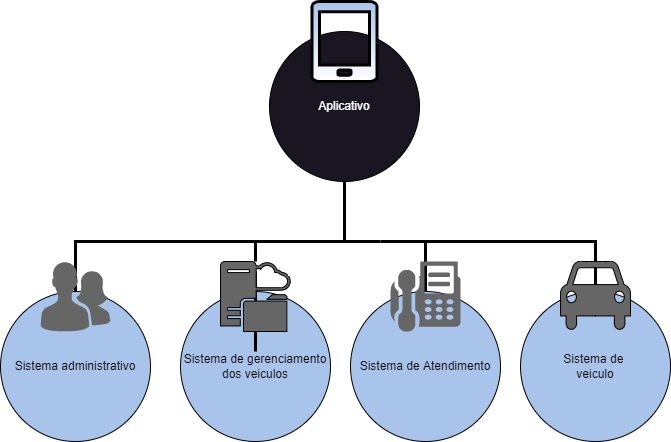
\includegraphics[width=15cm]{subsistemas.drawio.png} \\
      \end{center}
\end{figure}
\begin{figure}[H]
      \begin{center}
            \caption{ Diagrama de redes das Workstation} \label{afp}
            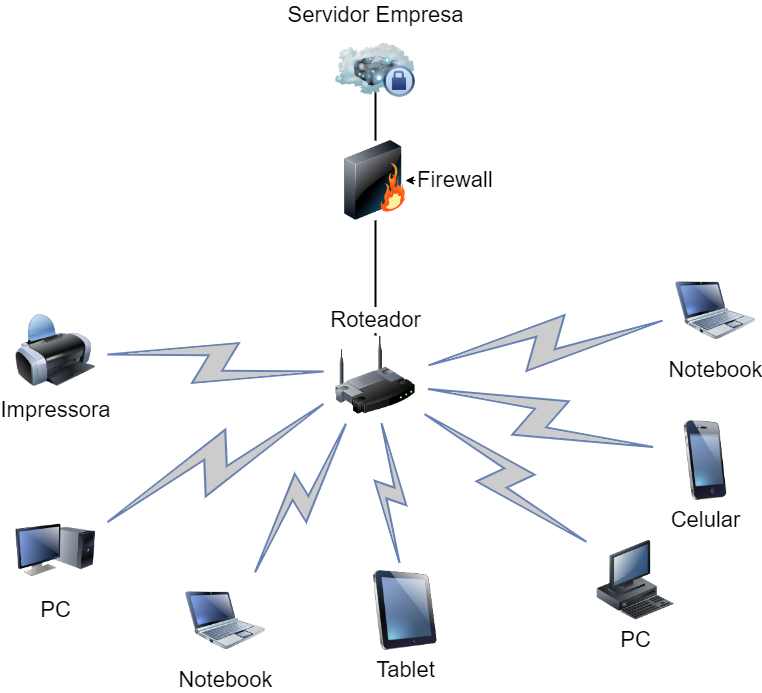
\includegraphics[width=15cm]{redeDiagram.drawio.png} \\
      \end{center}
\end{figure}

%%%%%%%%%%%%%%%%%%%%%%%%%%%%%%%%%%%%%%%


\section{Stakeholders e Pontos de Vista}
Esta seção apresenta as partes interessadas e pontos de vista mais importantes sobre o sistema.
\subsection{Stakeholders}

\begin{itemize}
      \item \textbf{Clientes;}
            \subitem - Usuários que fazem uso do sistema.
      \item \textbf{ Acionistas;}
            \subitem - Grupo de pessoas que investem no futuro da empresa.
      \item \textbf{Departamento de Inteligencia Artificial;}
            \subitem - Grupo de funcionários que desenvolve a essencial da empresa.
      \item \textbf{ Setor Administrativo;}
            \subitem - Equipe que faz a gestão de todos os funcionários da empresa.
      \item  \textbf{ Setor de desenvolvimento de software;}
            \subitem - Responsáveis pelo o desenvolvimento dos sistema interno da empresa, e Aplicativo.
      \item \textbf{ Departamento de marketing;}
            \subitem - Responsáveis pelo marketing e divulgação da empresa digitalmente.
      \item \textbf{ Setor de suporte ao cliente;}
            \subitem - Equipe de terceirizada que irão receber treinamento para fornecer suporte aos clientes da empresa.
      \item \textbf{ Representantes de terceirizadas.}
            \subitem - Grupo de empresas definidas que irão prestar serviços para a empresa.
\end{itemize}



\subsection{Pontos de vista}

Cada ponto de vista apresentado a seguir, seja ele direto ou indireto, está relacionado ao sistema.
\subsubsection{ Diretos}
\begin{itemize}
      \item \textbf{Cliente do aplicativo}\\
            Cadastro\\
            -Agendamento corrida\\
            -Resultados das corridas por aplicativo\\
            -Acompanhamento em tempo real da viagem\\
            -Pagamento da corrida\\

      \item \textbf{Funcionários}\\
            -Ponto pelo sistema\\
            -Interface amigável\\
            -Emissão de relatórios\\
            -Acesso autorizado\\
            -Gerenciamento de dados\\

      \item \textbf{Equipe de manutenção}\\
            -Manutenção de equipamentos\\
            -Manutenção de computadores\\
            -Manutenção de rede\\
            -Instalação de softwares\\
            -Instalação de equipamentos\\

      \item \textbf{Equipe do projeto}\\
            -Coleta de Requisitos\\
            -Desenvolvimento\\
            -Treinamento\\
            -Teste com usuários\\
            -Implementação\\

      \item \textbf{Equipe de IA}\\
            -Coleta de Requisitos\\
            -Desenvolvimento\\
            -Inteligencia Artificial\\
            -Implementação de recursos autônomos\\


      \item \textbf{Engenheiros de rede}\\
            -Servidores\\
            -Gerenciamento de rede\\
            -Segurança de rede\\

\end{itemize}
\subsubsection{ Indiretos}

\begin{itemize}
      \item \textbf{Setor Administrativo}\\
            -Receitas e despesas\\
            -Relatórios\\
            -Fornecedores\\
            -Dividas\\
            -Situação financeira\\


      \item \textbf{Direção geral da empresa}\\
            -Gerenciamento de recursos\\
            -Relatorio geral\\
            -Relatório de todos os setores\\
            -Gerenciamento de Funcionários\\
            -Contas a pagar\\


      \item \textbf{Fornecedores}\\
            -Recebimento de recursos\\
            -Acesso no Sistema na área de fornecedor\\
            -Acompanhamento de manutenções\\
            -Relatório de pagamentos\\





      \item \textbf{Acionistas}\\
            -Relatórios de ganhos\\
            -Situação financeira\\
            -Informações de todos os setores\\
            -Pedido de convocação de reunião\\
            -Gerenciamento de reuniões\\



      \item \textbf{Departamento de marketing}\\
            -Campanhas\\
            -Propagandas Publicitarias\\
            -Relatórios das campanhas\\
            -Pesquisas de Opinião\\
            -Estratégias para atrair pacientes\\
            -Análise de tendências\\
            -Elaboração de promoções\\
\end{itemize}



\subsection{ Hierarquia de pontos de vista}
Na figura \ref{vista} os pontos de vista são apresentados hierarquicamente de acordo com as prioridades do sistema, e os pontos de vista também são organizados de forma direta e indireta.
\begin{figure}[H]
      \begin{center}
            \caption{Hierarquia de pontos de vista} \label{vista}
            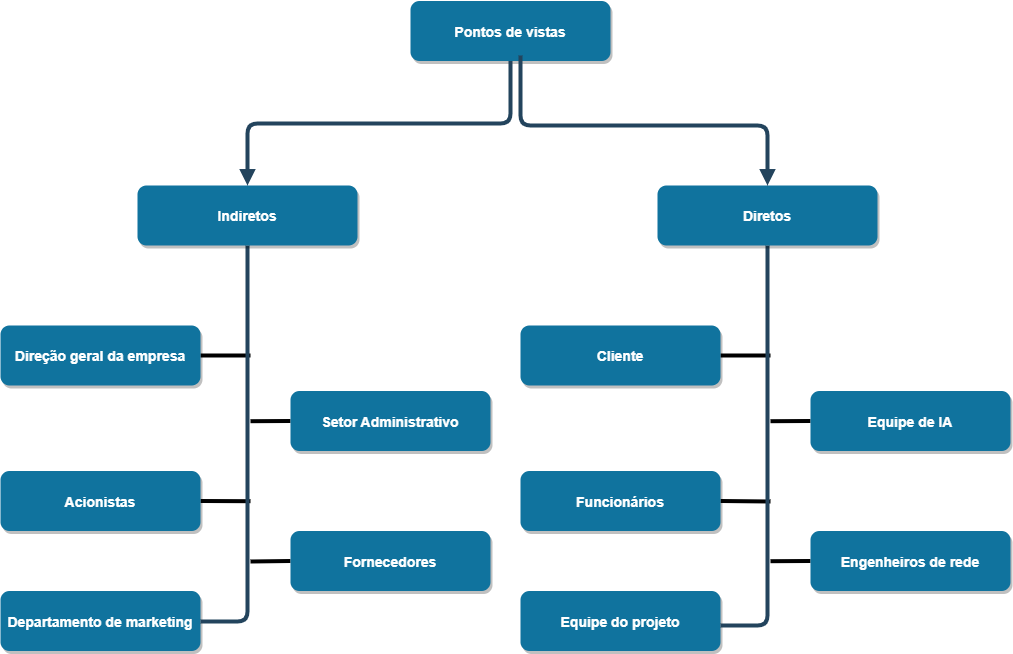
\includegraphics[width=15cm]{Untitled Diagram.drawio.png} \\

      \end{center}
\end{figure}

\section{Entrevista}



A entrevista é uma técnica fundametal e o método mais comumente usado para elicitar requisitos para um sistema. Foram selecionadas oito questões a serem feitas para o desenvolvimento do sistema de gestão de veículos. A entrevista é realizada com um funcionário da área de inteligência artificial e design de sistemas. O funcionário dos departamentos de inteligência artificial e design foi escolhido por possuir o maior conhecimento do sistema.  \\

\begin{enumerate}
      \item \textbf{O que você acha dos sistemas dos concorrentes?}
            \\R:Acho que os sistemas do concorrente estão desatualizados, pois não se encaixam no mundo em que vivemos atualmente. O sistema não oferece nenhum tipo de comodidade para clientes e colaboradores, o que acaba dificultando a captação de novos clientes e o atendimento e atendimento de veículos direto aos mesmos .\\

      \item \textbf{No sistema de qual forma os clientes solicitam corridas? Como você analisa essa forma de auto-atendimento?}
            \\R:Eu acho que é um sistema útil, pois se adapta ao mundo em que vivemos. O sistema não impõe restrições a funcionários e clientes, e isso não dificulta a captação e atendimento de novos clientes. \\

      \item \textbf{Quais são alguns dos problemas que os clientes podem enfrentar diariamente?}
            \\R: A única forma de solicitar veículos e as muitas funcionalidades que o sistema oferece podem limitar sua aplicação para alguns clientes. Por exemplo: no sistema existe a função de pagar com cartão, e outra função que ele tem é a variedade de opções para o paciente ir junto, já que atualmente as caronas só são possíveis no aplicativo. \\

      \item \textbf{Quais melhorias você gostaria?}
            \\R: Como já mencionado, a diversidade na consulta e planejamento de viagens leva a filas de clientes. Outras melhorias incluíram uma escolha mais ampla de métodos de pagamento e outras maneiras de o cliente obter resultados de corrida em tempo real.\\

      \item \textbf{O que você acha da interface do sistema do concorrente?}
            \\R:Não acho que seja intuitivo, pois a interface do usuário do sistema funciona por meio de linhas de comando, dificultando a compreensão do sistema para os novos funcionários. \\

      \item \textbf{O sistema atual dos concorrentes é fácil de usar?}
            \\R: Não, como mencionado anteriormente, o sistema não é intuitivo , o que dificulta o uso do sistema.\\

      \item \textbf{Os usuários concorrentes usam todos os recursos do sistema?}
            \\R: Não, existem alguns cuja funcionalidade desconheço, pois os dados coletados não mencionam o uso desses recursos pelos clientes do concorrente. \\

      \item \textbf{O que você acrescentaria ao sistema em relação aos concorrentes?}
            \\R:Eu acrescentaria a opção de agendar o ponto de espera dos veículos pelo próprio sistema, essa opção reduzirá a perda de tempo em relação aos concorrentes. Como resultado, seus clientes se mudam para o local onde os veículos estão localizados. Quando um cliente solicita um veículo no sistema, ele é automaticamente marcado em um local selecionado pelo usuário.
\end{enumerate}

\subsection{Relatório da entrevista}

A partir da entrevista, fica claro que o sistema atual dos concorrentes está desatualizado e não atende as necessidades dos clientes e colaboradores da empresa. Os principais problemas observados foram a falta de variedade de meios de pagamento, falta de meios para agilizar a reserva de viagens e a visualização eficiente e detalhada das viagens já realizadas. Também foi notada a falta de interatividade da interface, que funciona no sistema do concorrente com meios arcaicos e dificulta a adaptação de novos funcionários e clientes.

Observou-se também que os funcionários não conhecem as características de algumas funções do sistema, o que leva à não utilização de algumas funções. Isso se deve ao mau treinamento da equipe em relação ao sistema. O funcionário entrevistado sugeriu o agendamento de viagens pelo sistema com o objetivo de reduzir o tempo de deslocamento dos clientes até o local sugerido pelo aplicativo concorrente.



\section{ Casos de Uso}

Esta seção apresenta os casos de uso do sistema, cujo objetivo é mostrar as interações realizadas pelo usuário e as reações do sistema.

\subsection{Cadastro dos usuarios}
\begin{enumerate}
      \item Preenchimento dos dados cadastrais do usuários;
      \item Login no sistema;

      \item Verificação de dados;
      \item Confirmação de dados;
      \item Escolha do método de pagamento;
      \item Gerar informações do usuário;

      \item Gerar relatório do usuários;
      \item Finalizar cadastro.
\end{enumerate}

\subsection{ Cadastro de recursos de terceirizadas}
\begin{enumerate}
      \item Login da terceirizada no sistema;
      \item Preenchimento de dados do recurso fornecido pela terceirizada;
      \item Informar valor do recurso;
      \item Atualizar dados do sistema;
      \item Finalizar cadastro de novos dados;
      \item Gerar relatório atual.
\end{enumerate}


\subsection{ Cadastro de novos funcionários}
\begin{enumerate}
      \item Gerar login do sistema;
      \item Preenchimento de dados pessoais do funcionário;
      \item Informa o setor;
      \item Informa o cargo;
      \item Calcular salário inicial;
      \item Preencher informações de pagamento de salário;
      \item Gerar ID do funcionário;
      \item Finalizar cadastro;
      \item Gerar relatório.

\end{enumerate}

\subsection{ Diagrama de Caso de Uso}
O diagrama a seguir pretende representar graficamente o caso de um "Serviço a um Usuário".
Cujo tem como objetivo representar o caso de uso do sistema e exibir informações sobre ele.

\begin{figure}[H]
      \begin{center}
            \caption{ Diagrama de caso de uso de um Serviço a um Usuário} \label{afp}
            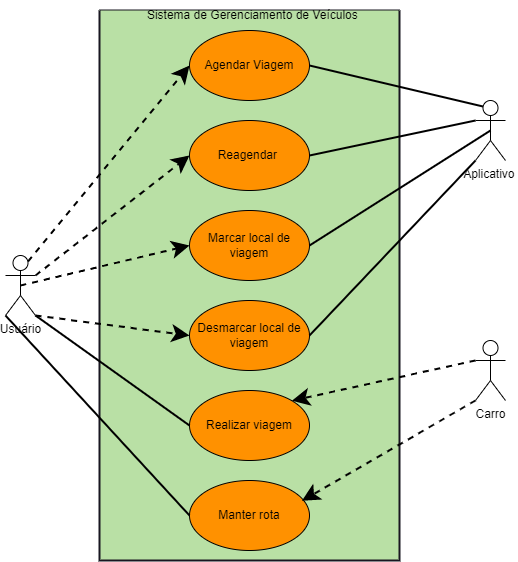
\includegraphics[width=15cm]{casodeuso.drawio.png} \\


      \end{center}
\end{figure}








\section{Modelagem do Sistema}
Nesta seção será apresentado a modelagem do sistema. Assim como os seus diagramas de contexto, diagramas do sistema, diagramas de processos, modelagem de dados, e diagramas de entidades de relacionamentos.


\subsection{Diagrama de contexto}
O diagrama de contexto destina-se a representar todo o sistema de maneira ampla, genérica e objetiva para orientar o propósito geral do sistema. O mesmo pode ser visto na figura \ref{contexto}.
\begin{figure}[H]
      \begin{center}
            \caption{Diagrama de contexto} \label{contexto}
            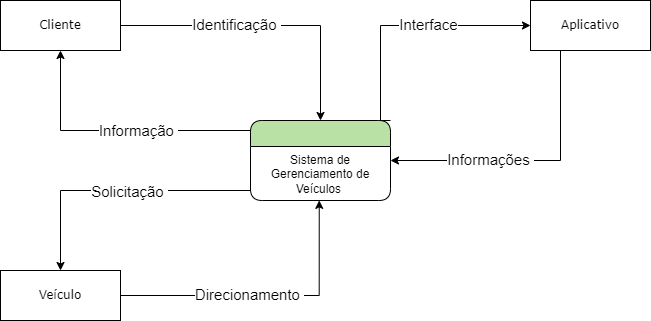
\includegraphics[width=15cm]{systemDiagram.drawio.png} \\
      \end{center}
\end{figure}

\subsection{Diagrama do sistema}
O diagrama do sistema \ref{siste} tenta representar graficamente o sistema geral com todos os seus processos, subdivisões, fluxos de dados e bancos de dados de uma maneira mais específica para cobrir todos os pontos importantes do sistema.

\begin{figure}[H]
      \begin{center}
            \caption{Diagrama de fluxo de dados do sistema} \label{siste}
            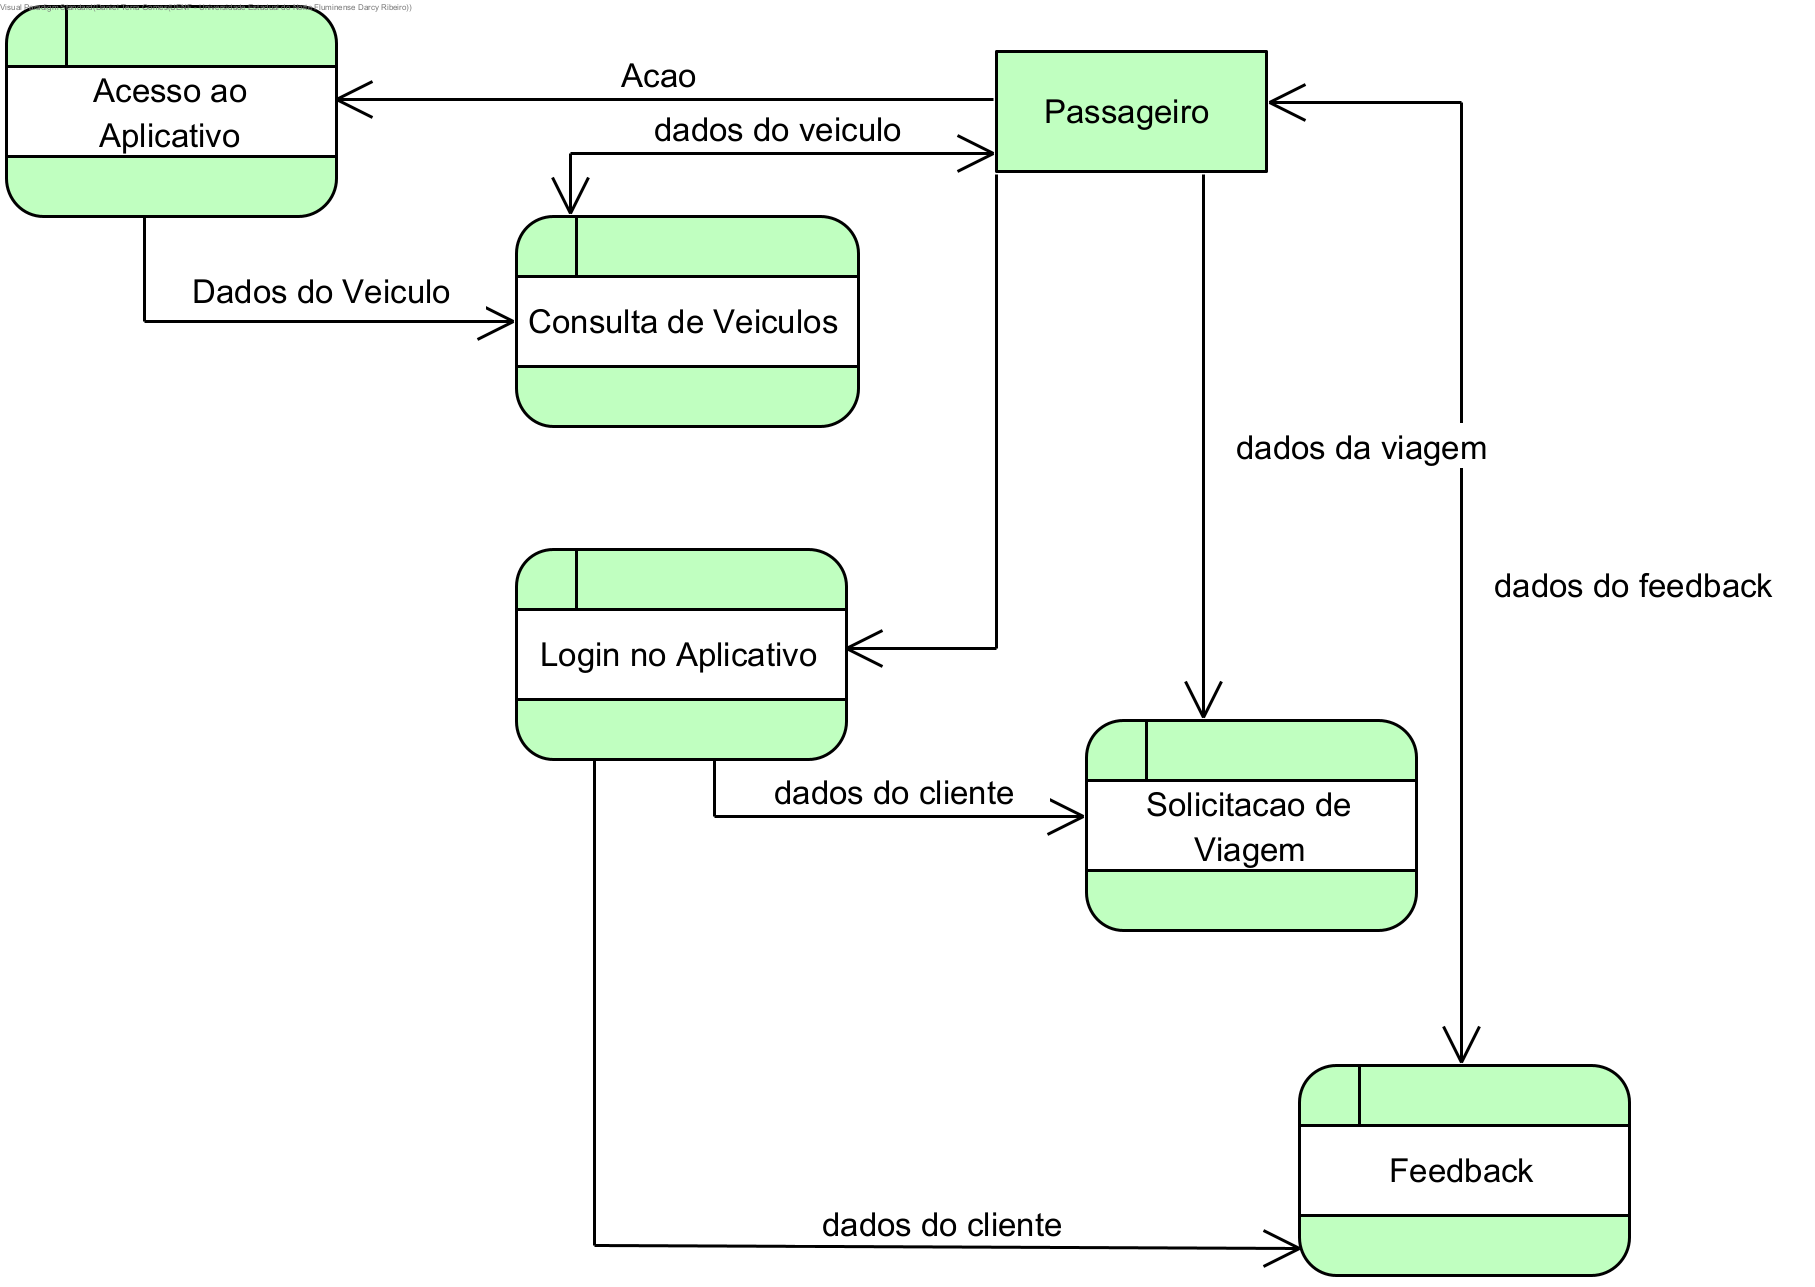
\includegraphics[width=15cm]{sistema.png} \\

      \end{center}
\end{figure}


\subsection{Diagramas de processos}
Nesta seção são apresentados diagramas de alguns processos específicos, com o intuito de ter uma
visão mais próxima do funcionamento dos mesmos.

\textbf{Gerenciamento de Veículos}

O processo de gerenciamento de veículos na figura \ref{gerenciamento} é utilizado pelo aplicativo e possui funções como: visualizar, alterar, solicitar e assim por diante.


\begin{figure}[H]
      \begin{center}
            \caption{Diagrama do sistema nivel 1} \label{gerenciamento}
            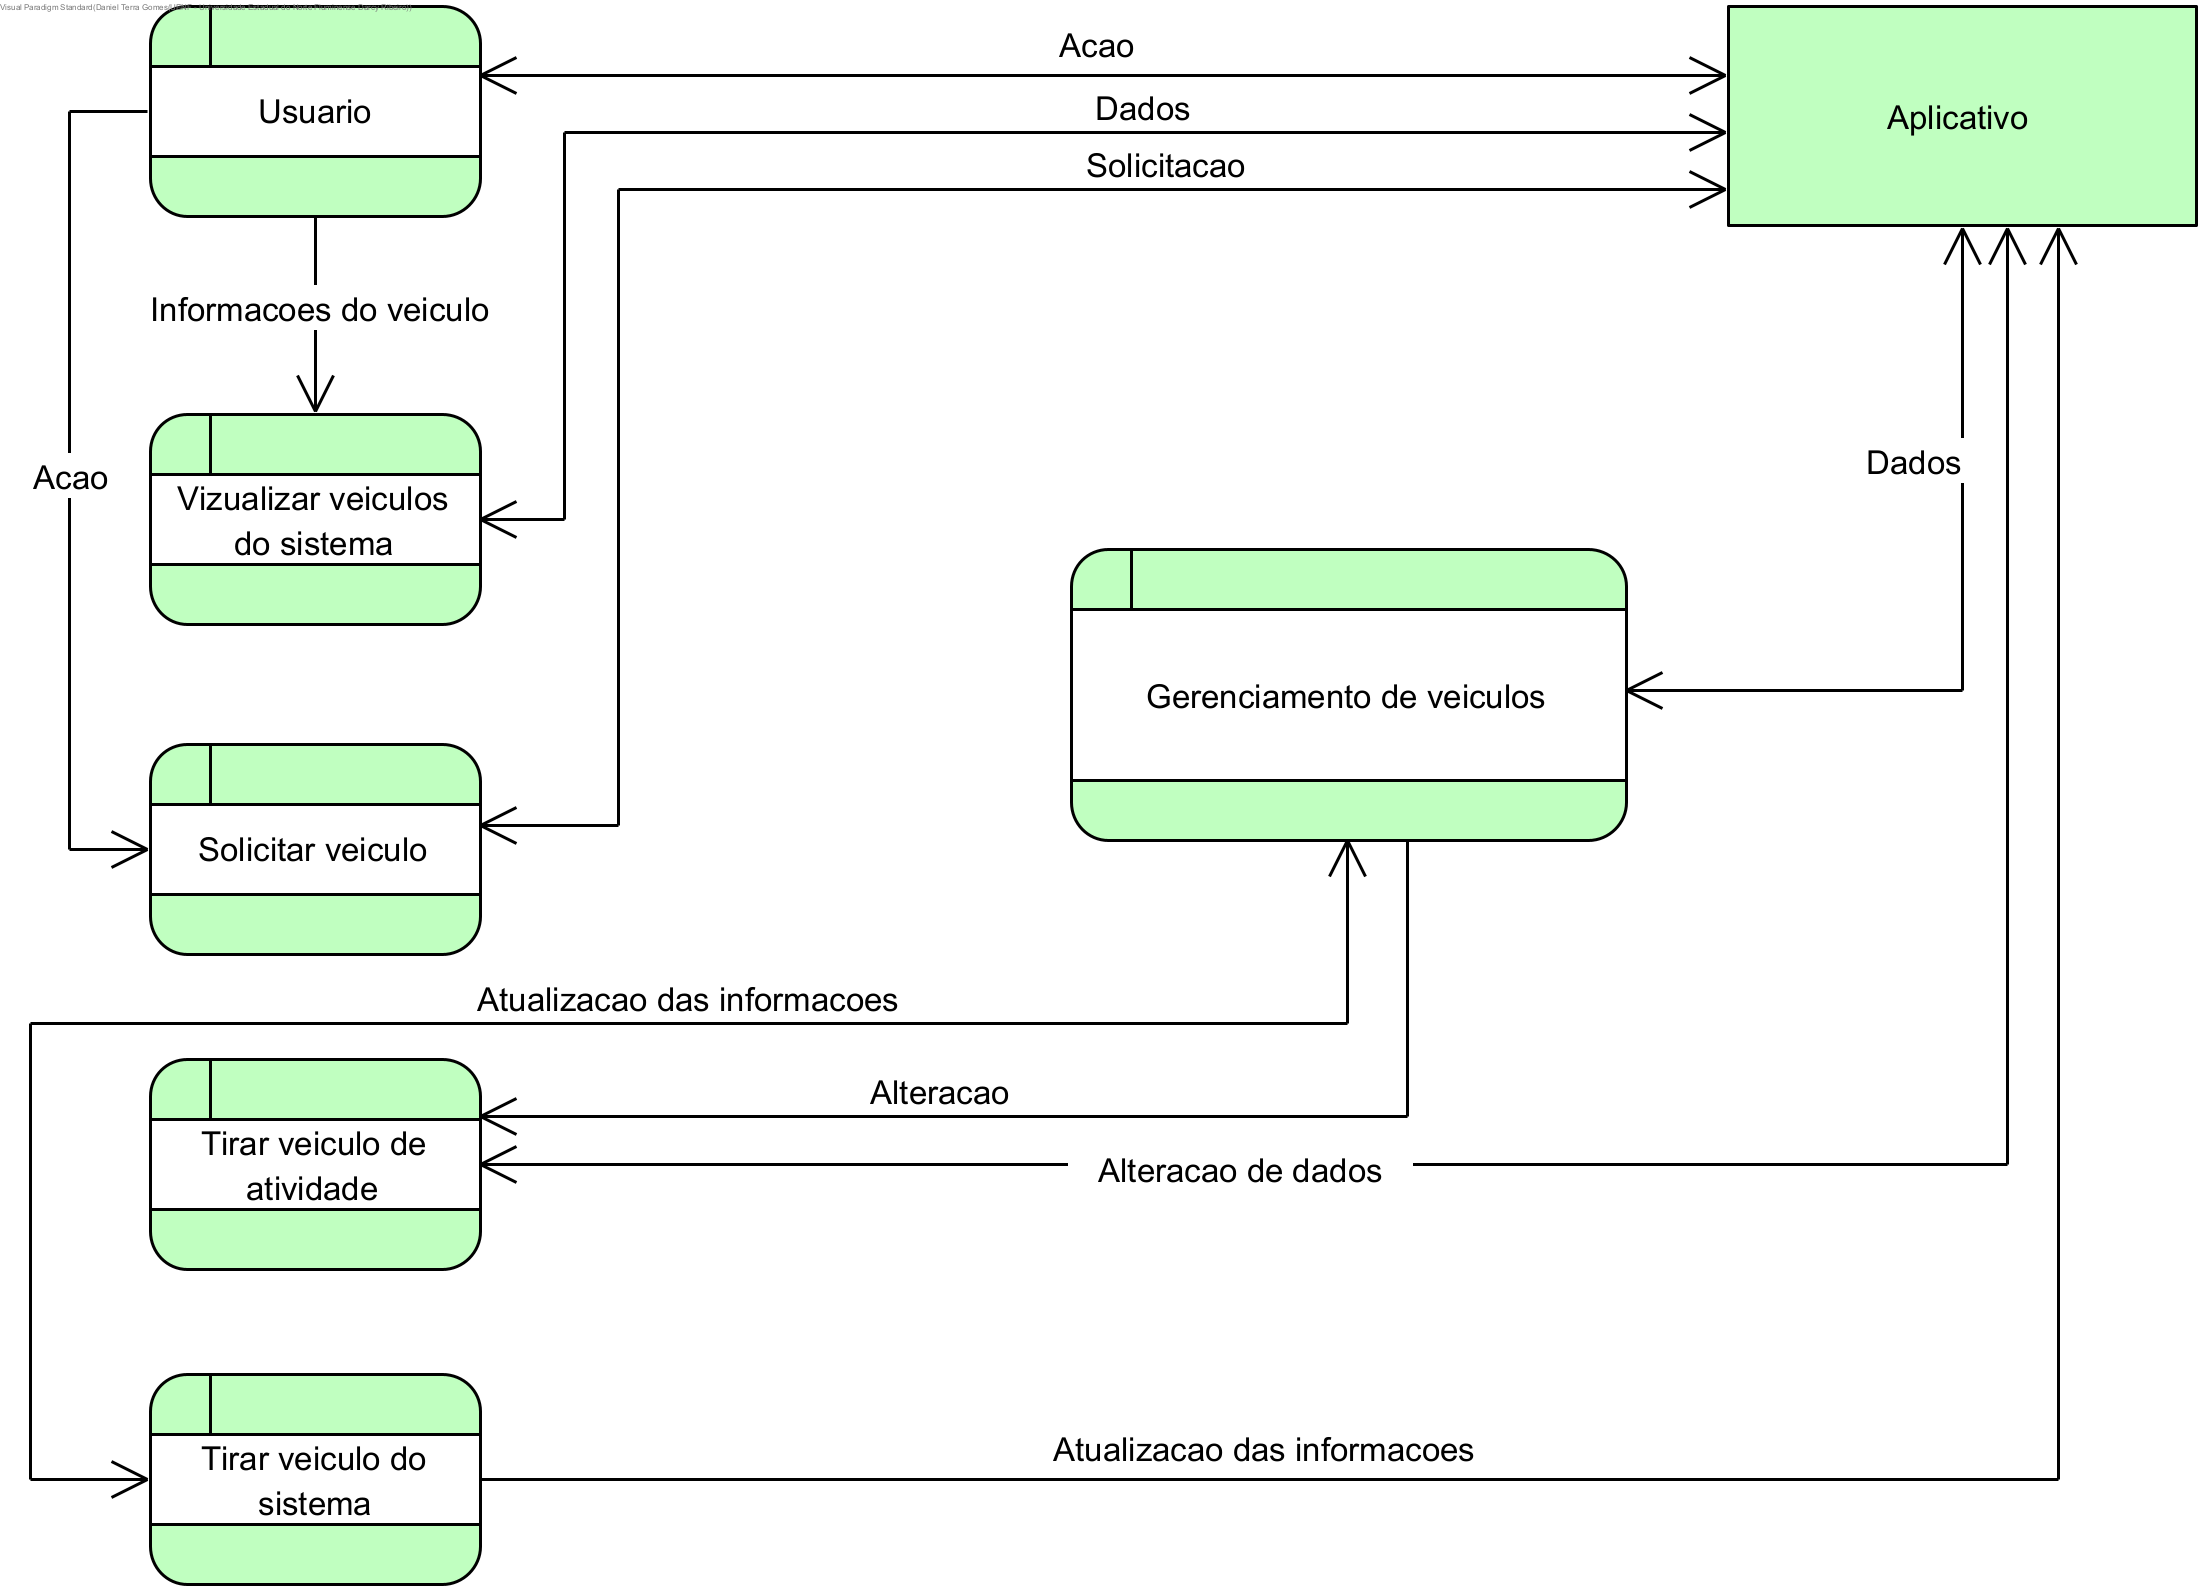
\includegraphics[width=15cm]{gerenciamento.png} \\

      \end{center}
\end{figure}


%%%%%%%%%%%%%%%%%%%%%%%






%%%%%%%%%%%%%%%%%%%%%%%
\subsection{Modelagem de Dados}
A seção a seguir mostra os diagramas destinados a modelar o relacionamento entre entidades. São apresentados 4 diagramas de relacionamento: diagrama cliente-entidade no aplicativo \ref{aplicativo}, Acidente com veículo da empresa \ref{acidente},  subsistema de Manutenção de veiculo \ref{manutencao} e diagrama de entidade da avaliação do usuário \ref{avaliacao} .
\subsection{Diagramas de entidades e relacionamentos}
Diagramas de Fluxo de Dados é uma forma de representar graficamente as relações entre os processos e as bases de dados do sistema.

\begin{figure}[H]
      \begin{center}
            \caption{Diagrama de entidade: solicitação de veículo no aplicativo} \label{aplicativo}
            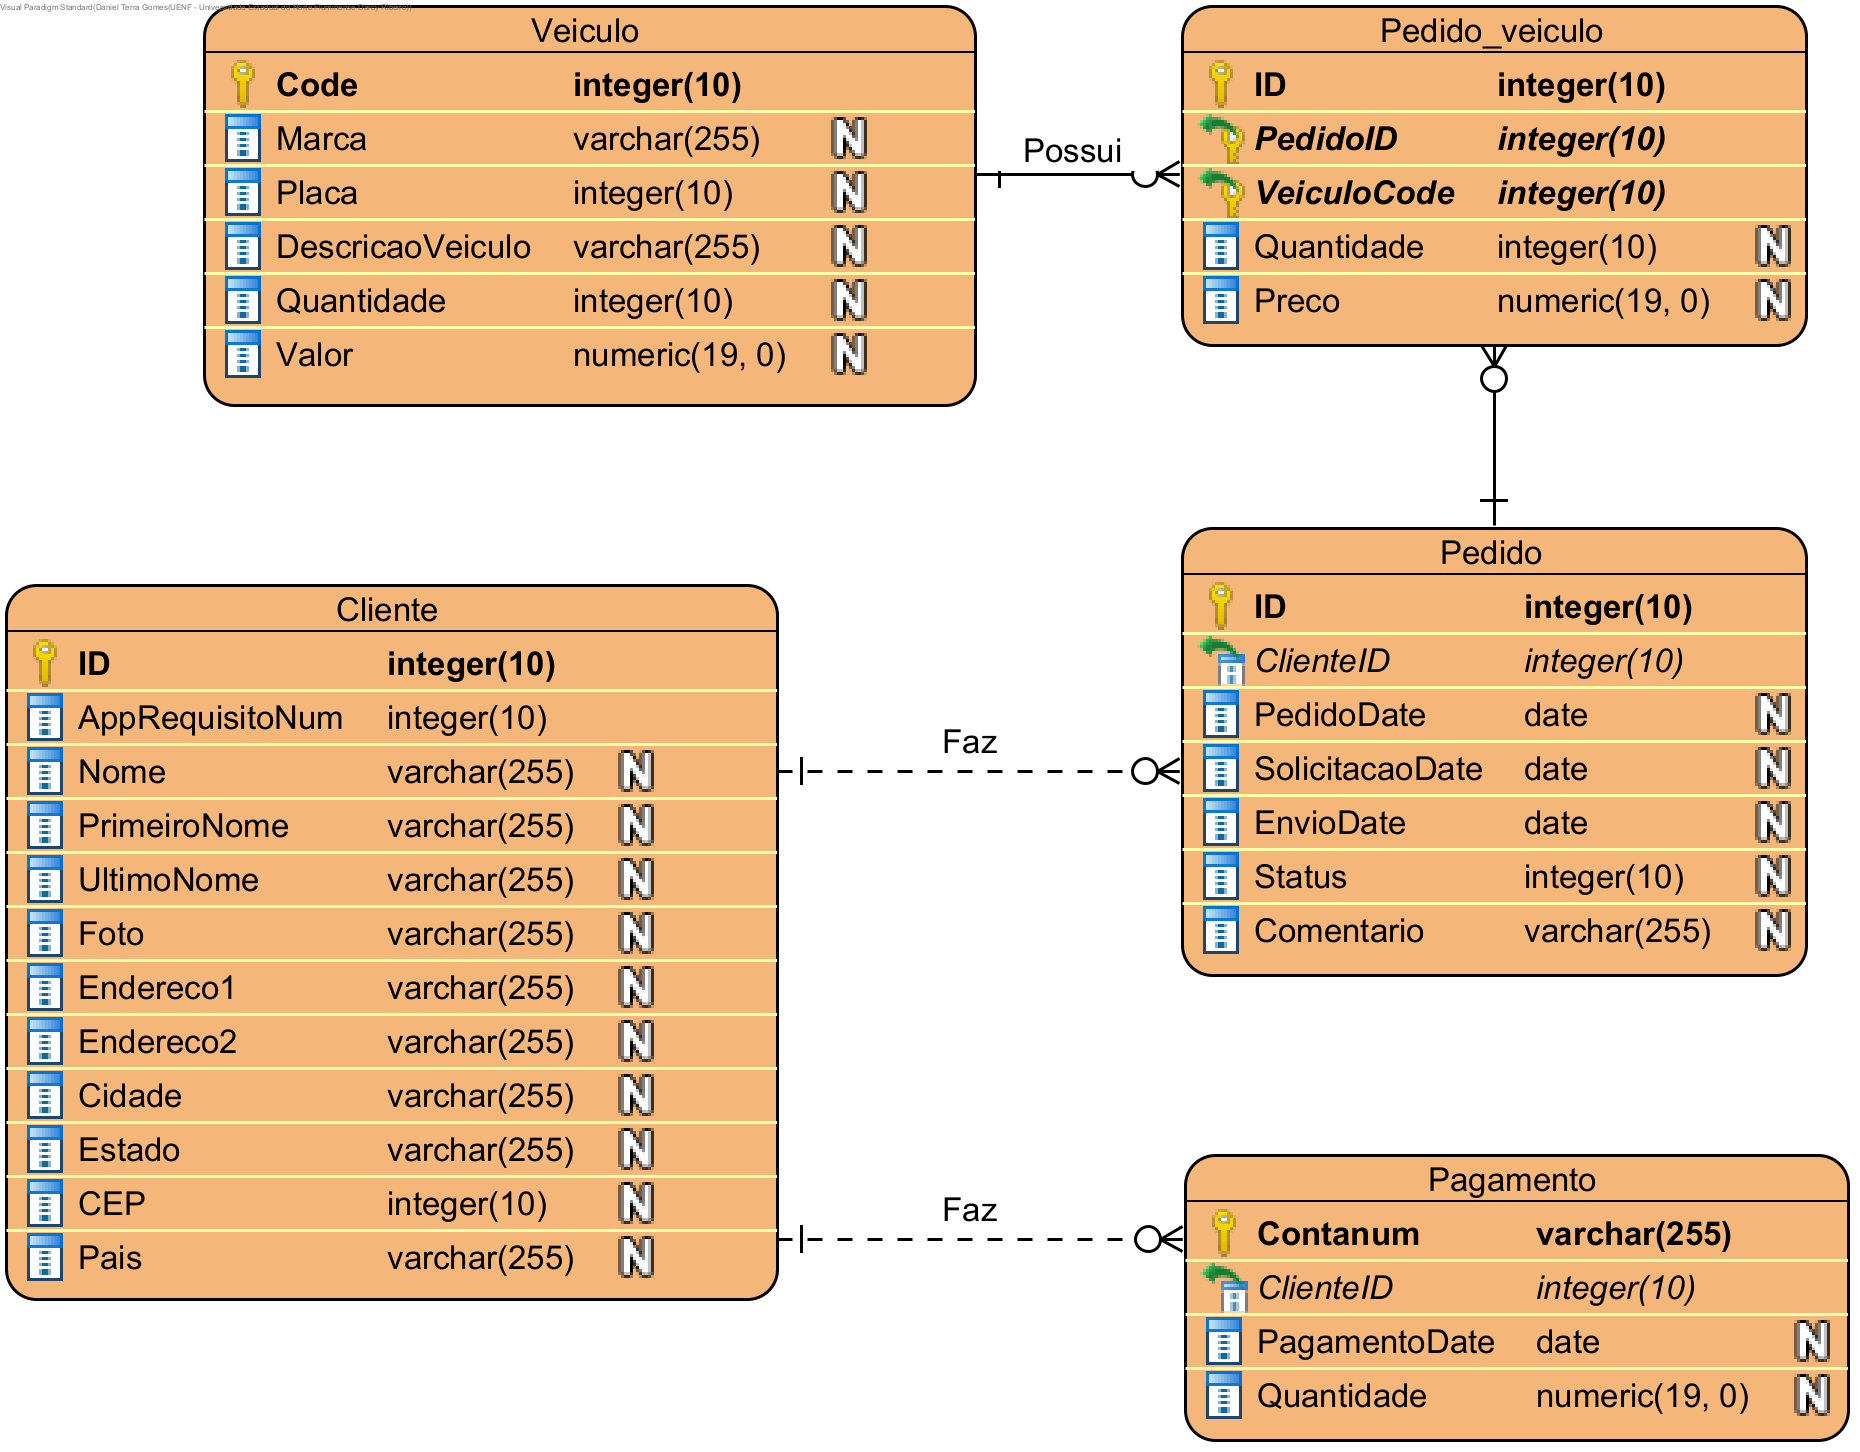
\includegraphics[width=15cm]{cliente.png} \\

      \end{center}
\end{figure}


\begin{figure}[H]
      \begin{center}
            \caption{Diagrama de entidade: acidente com veículo da empresa} \label{acidente}
            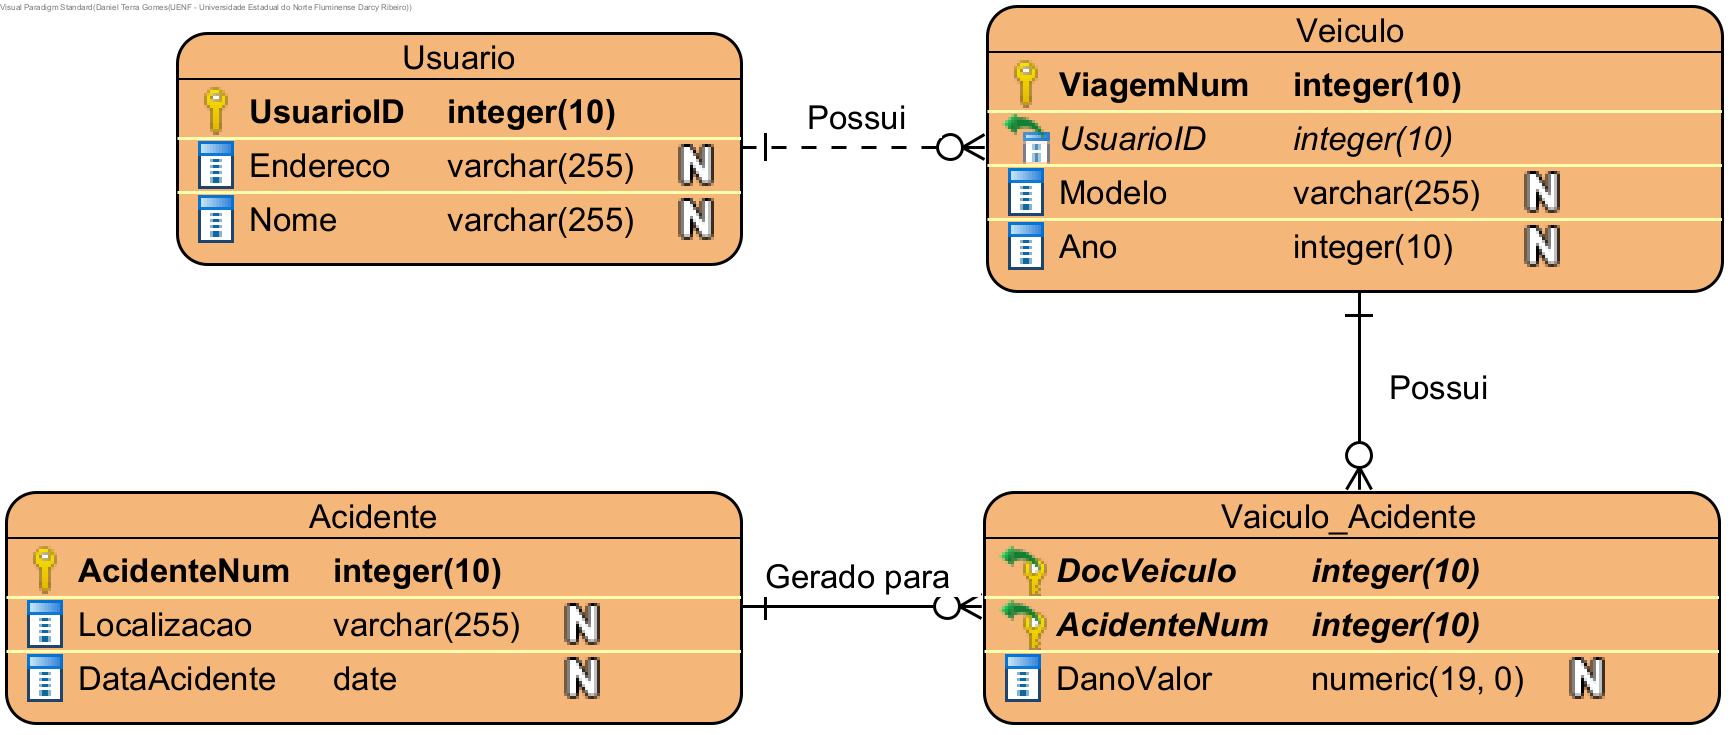
\includegraphics[width=12cm]{acidente.png} \\

      \end{center}
\end{figure}

\begin{figure}[H]
      \begin{center}
            \caption{Diagrama de entidade: manutenção de veiculos da empresa} \label{manutencao}
            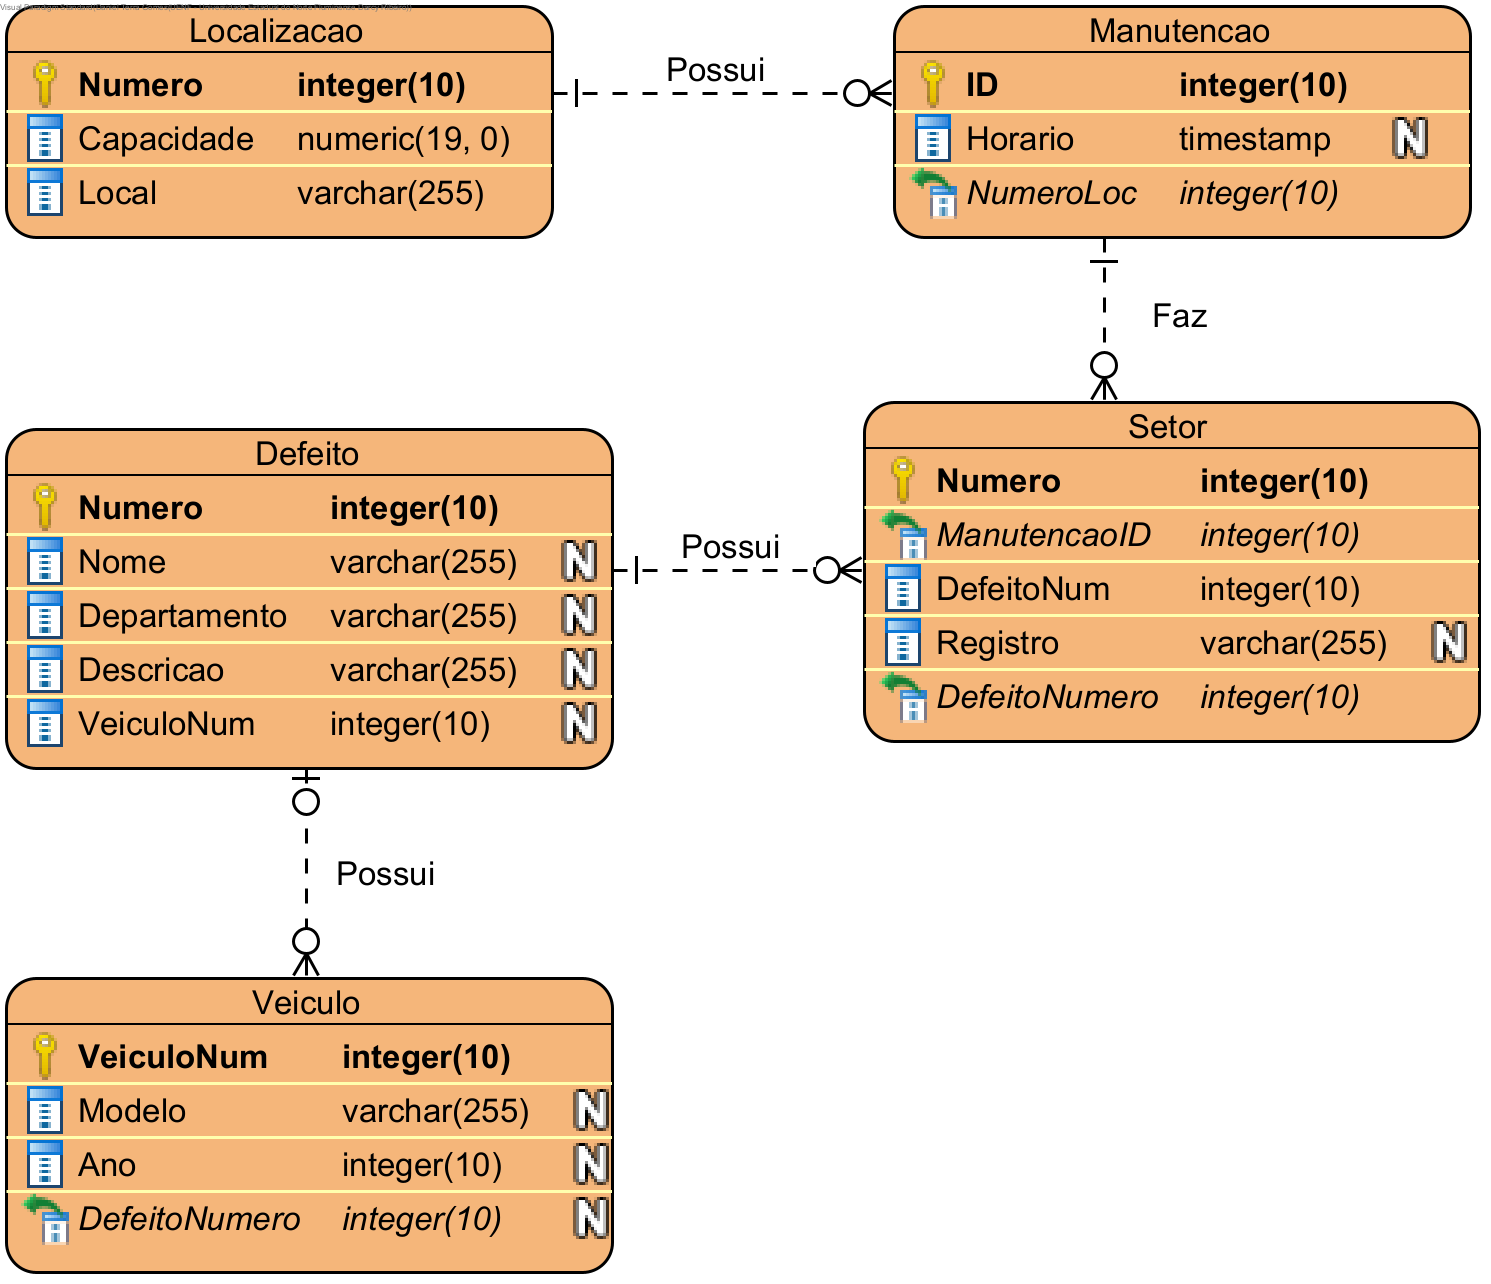
\includegraphics[width=15cm]{manutencao.png} \\

      \end{center}
\end{figure}

\begin{figure}[H]
      \begin{center}
            \caption{Diagrama de entidade: avaliação do usuario} \label{avaliacao}
            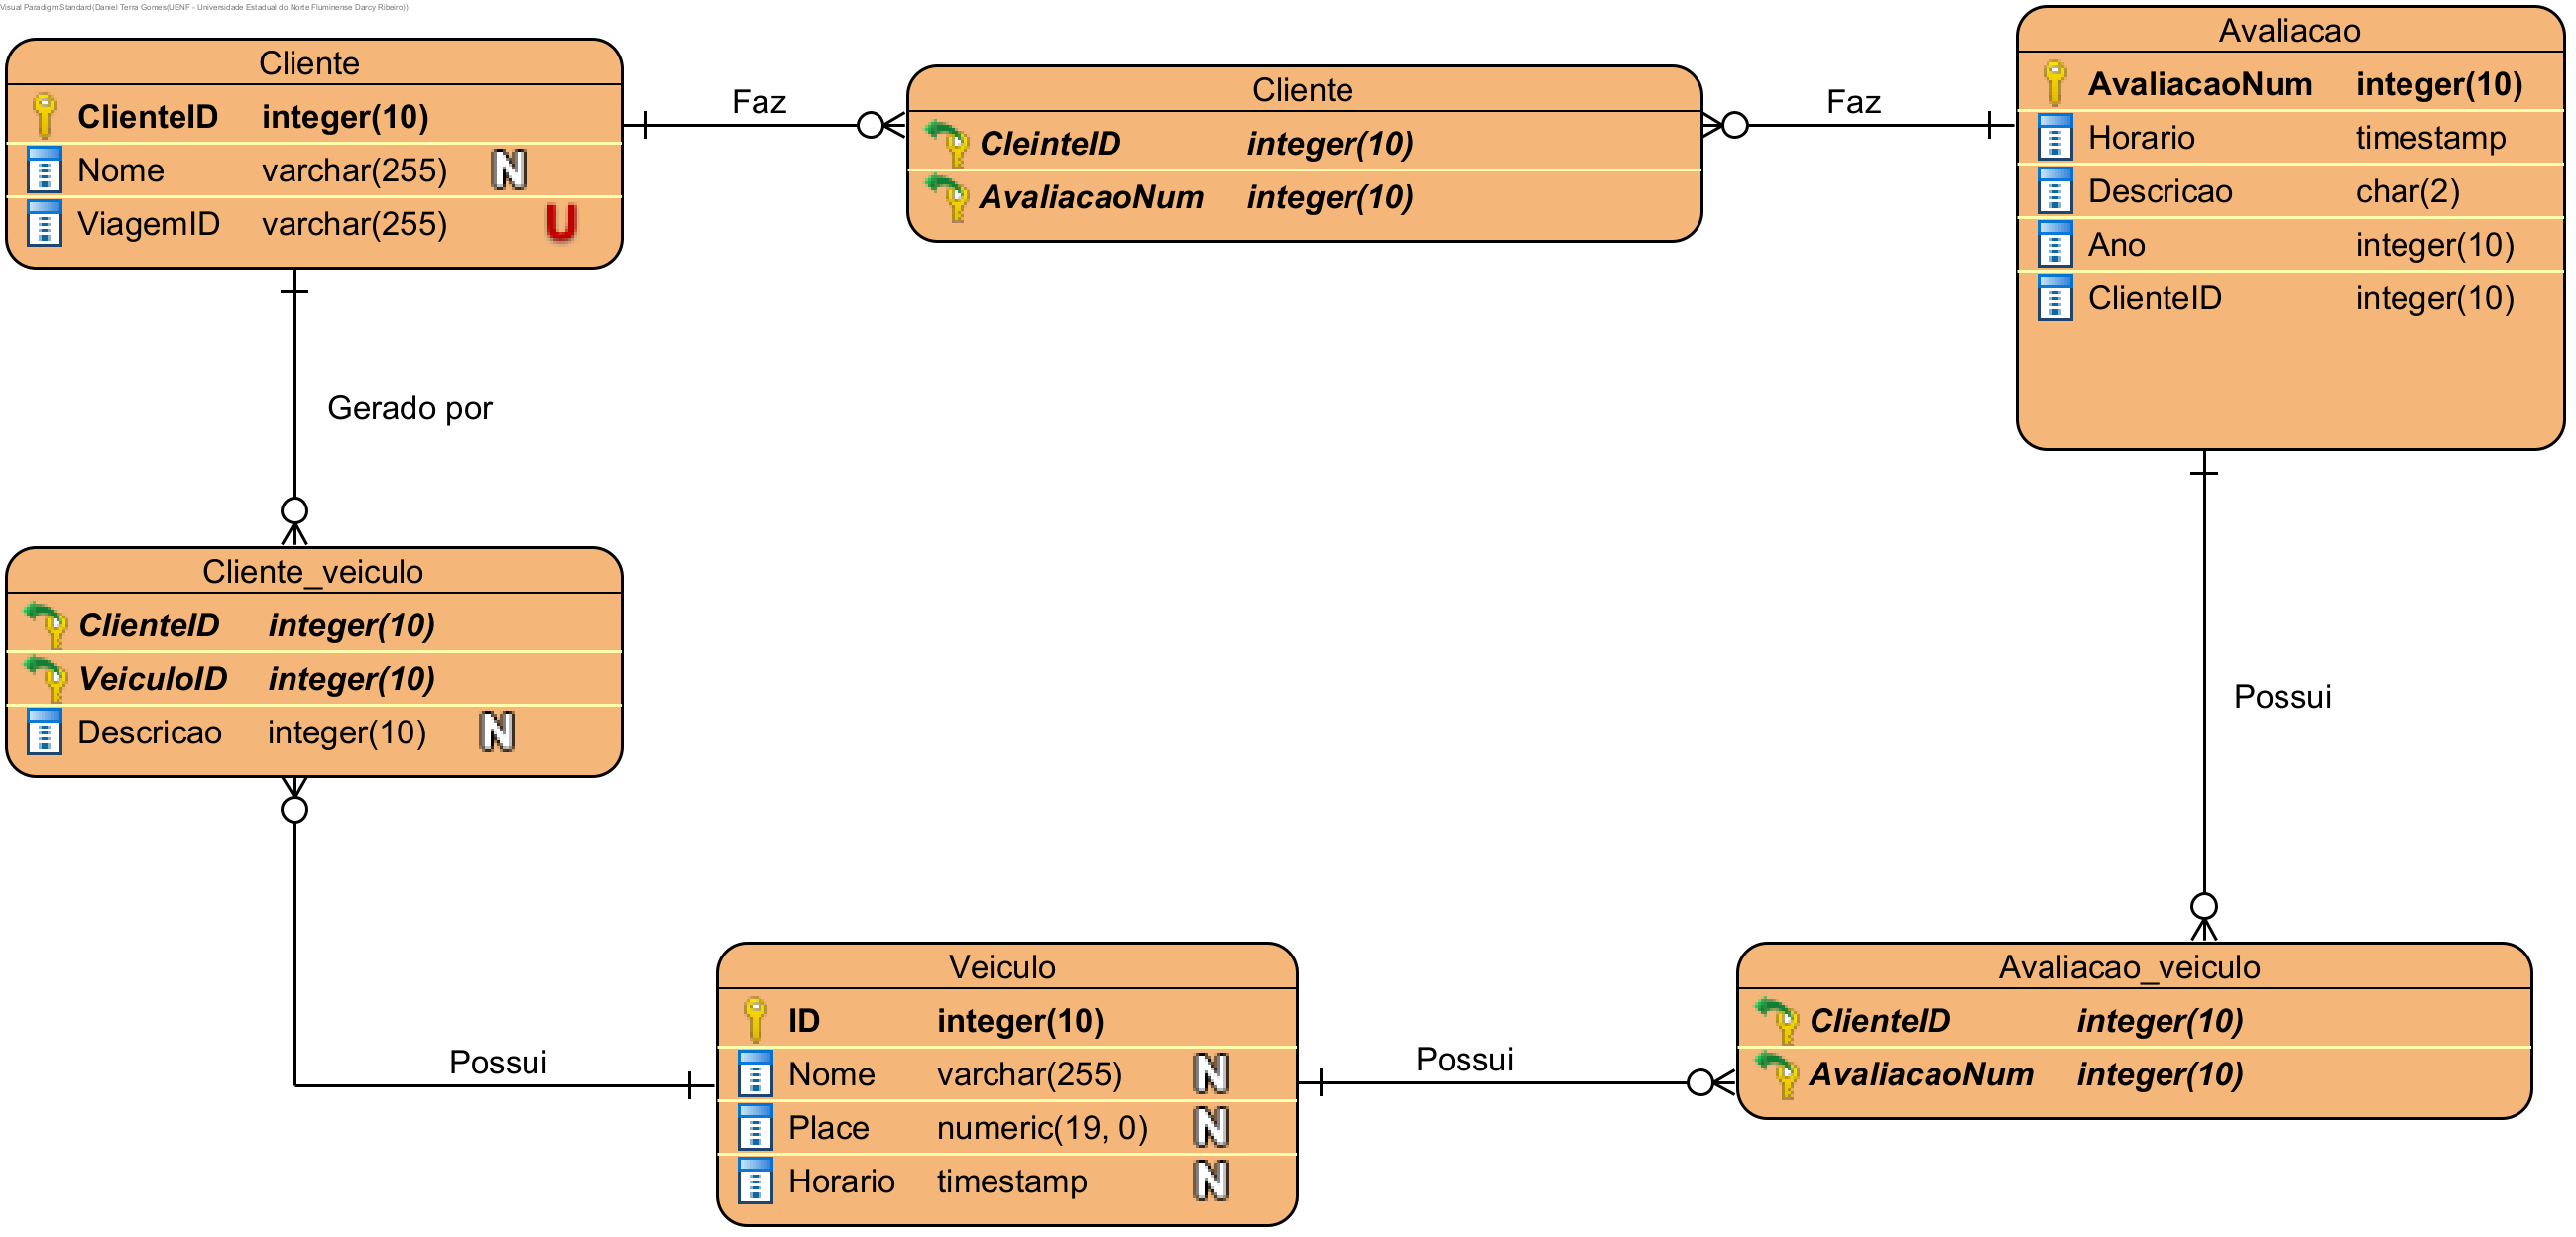
\includegraphics[width=15cm]{avaliacao.png} \\
      \end{center}
\end{figure}
